% Options for packages loaded elsewhere
\PassOptionsToPackage{unicode}{hyperref}
\PassOptionsToPackage{hyphens}{url}
%
\documentclass[
]{article}
\usepackage{amsmath,amssymb}
\usepackage{iftex}
\ifPDFTeX
  \usepackage[T1]{fontenc}
  \usepackage[utf8]{inputenc}
  \usepackage{textcomp} % provide euro and other symbols
\else % if luatex or xetex
  \usepackage{unicode-math} % this also loads fontspec
  \defaultfontfeatures{Scale=MatchLowercase}
  \defaultfontfeatures[\rmfamily]{Ligatures=TeX,Scale=1}
\fi
\usepackage{lmodern}
\ifPDFTeX\else
  % xetex/luatex font selection
\fi
% Use upquote if available, for straight quotes in verbatim environments
\IfFileExists{upquote.sty}{\usepackage{upquote}}{}
\IfFileExists{microtype.sty}{% use microtype if available
  \usepackage[]{microtype}
  \UseMicrotypeSet[protrusion]{basicmath} % disable protrusion for tt fonts
}{}
\makeatletter
\@ifundefined{KOMAClassName}{% if non-KOMA class
  \IfFileExists{parskip.sty}{%
    \usepackage{parskip}
  }{% else
    \setlength{\parindent}{0pt}
    \setlength{\parskip}{6pt plus 2pt minus 1pt}}
}{% if KOMA class
  \KOMAoptions{parskip=half}}
\makeatother
\usepackage{xcolor}
\usepackage[margin=1in]{geometry}
\usepackage{longtable,booktabs,array}
\usepackage{calc} % for calculating minipage widths
% Correct order of tables after \paragraph or \subparagraph
\usepackage{etoolbox}
\makeatletter
\patchcmd\longtable{\par}{\if@noskipsec\mbox{}\fi\par}{}{}
\makeatother
% Allow footnotes in longtable head/foot
\IfFileExists{footnotehyper.sty}{\usepackage{footnotehyper}}{\usepackage{footnote}}
\makesavenoteenv{longtable}
\usepackage{graphicx}
\makeatletter
\def\maxwidth{\ifdim\Gin@nat@width>\linewidth\linewidth\else\Gin@nat@width\fi}
\def\maxheight{\ifdim\Gin@nat@height>\textheight\textheight\else\Gin@nat@height\fi}
\makeatother
% Scale images if necessary, so that they will not overflow the page
% margins by default, and it is still possible to overwrite the defaults
% using explicit options in \includegraphics[width, height, ...]{}
\setkeys{Gin}{width=\maxwidth,height=\maxheight,keepaspectratio}
% Set default figure placement to htbp
\makeatletter
\def\fps@figure{htbp}
\makeatother
\setlength{\emergencystretch}{3em} % prevent overfull lines
\providecommand{\tightlist}{%
  \setlength{\itemsep}{0pt}\setlength{\parskip}{0pt}}
\setcounter{secnumdepth}{5}
\newlength{\cslhangindent}
\setlength{\cslhangindent}{1.5em}
\newlength{\csllabelwidth}
\setlength{\csllabelwidth}{3em}
\newlength{\cslentryspacingunit} % times entry-spacing
\setlength{\cslentryspacingunit}{\parskip}
\newenvironment{CSLReferences}[2] % #1 hanging-ident, #2 entry spacing
 {% don't indent paragraphs
  \setlength{\parindent}{0pt}
  % turn on hanging indent if param 1 is 1
  \ifodd #1
  \let\oldpar\par
  \def\par{\hangindent=\cslhangindent\oldpar}
  \fi
  % set entry spacing
  \setlength{\parskip}{#2\cslentryspacingunit}
 }%
 {}
\usepackage{calc}
\newcommand{\CSLBlock}[1]{#1\hfill\break}
\newcommand{\CSLLeftMargin}[1]{\parbox[t]{\csllabelwidth}{#1}}
\newcommand{\CSLRightInline}[1]{\parbox[t]{\linewidth - \csllabelwidth}{#1}\break}
\newcommand{\CSLIndent}[1]{\hspace{\cslhangindent}#1}
\usepackage{caption} \usepackage{booktabs} \usepackage{xcolor} \usepackage{longtable} \usepackage{float} \usepackage{rotating} \floatplacement{figure}{H} \usepackage{lineno} \usepackage{pdfpages} \linenumbers
\usepackage{booktabs}
\usepackage{longtable}
\usepackage{array}
\usepackage{multirow}
\usepackage{wrapfig}
\usepackage{float}
\usepackage{colortbl}
\usepackage{pdflscape}
\usepackage{tabu}
\usepackage{threeparttable}
\usepackage{threeparttablex}
\usepackage[normalem]{ulem}
\usepackage{makecell}
\usepackage{xcolor}
\ifLuaTeX
  \usepackage{selnolig}  % disable illegal ligatures
\fi
\IfFileExists{bookmark.sty}{\usepackage{bookmark}}{\usepackage{hyperref}}
\IfFileExists{xurl.sty}{\usepackage{xurl}}{} % add URL line breaks if available
\urlstyle{same}
\hypersetup{
  pdftitle={Achieving universal energy access while reducing energy demand? Evidence from energy-specific population projections},
  pdfauthor={Camille Belmin\^{}1\^{}2\^{}3; Peter-Paul Pichler\^{}1; Guillaume Marois \^{}3\^{}4; Shonali Pachauri\^{}3; Helga Weisz\^{}1\^{}2},
  hidelinks,
  pdfcreator={LaTeX via pandoc}}

\title{Achieving universal energy access while reducing energy demand? Evidence from energy-specific population projections}
\author{Camille Belmin\(^1\)\(^2\)\(^3\) \and Peter-Paul Pichler\(^1\) \and Guillaume Marois \(^3\)\(^4\) \and Shonali Pachauri\(^3\) \and Helga Weisz\(^1\)\(^2\)}
\date{}

\begin{document}
\maketitle

\(^1\) Potsdam Institute for Climate Impact Research, Germany\\
\(^2\) Humboldt University Berlin, Germany\\
\(^3\) International Institute for Applied Systems Analysis, Wittgenstein Center (IIASA, OeAW, University of Vienna), Austria\\
\(^4\) Asian Demographic Research Institute of the Shanghai University, China

\hypertarget{abstract}{%
\section*{Abstract}\label{abstract}}
\addcontentsline{toc}{section}{Abstract}

In a climate- constrained world, understanding the energy required to achieve universal access to modern energy is critical. This requires making assumptions on future population trajectories, but the extent of energy access can affect these. Yet, this feedback has never been accounted for in energy models. Access to modern energy leads to fertility declines as it reduces child mortality, improves health, increases women's access to information, education and employment. In this paper, we assessed the household energy requirements to expand energy access while considering the relationship between energy access and fertility, using Zambia as a case study. To do so, we built a microsimulation model to project population, accounting for how fertility depends on access to modern energy and education. We used these population projections to then estimate household energy demand of the Zambian population until 2070, under different scenarios. We found that in 2070, while electricity consumption is higher in a universal access scenario compared to a baseline scenario, total energy demand is 29\% lower, partly due to a strong decline in the use of inefficient traditional cooking fuels. We also found that reduced population growth due to universal energy access contributes to lowering the energy demand by 55\% by 2050, compared to a more limited expansion in energy access, and this contribution increases over time. Although the challenge of achieving universal access to modern energy seems daunting, our results suggest that this could have co-benefits with achieving climate goals. Our study also reveals that accounting for the energy-population nexus in energy models will scale down the currently assumed energy needs to ensure a decent life for all.

\newpage

\hypertarget{intro}{%
\section{Introduction}\label{intro}}

Access to modern energy provides services that are essential to fulfill basic human needs (\protect\hyperlink{ref-gea_global_2012}{GEA 2012}; \protect\hyperlink{ref-mccollum_connecting_2018}{McCollum et al. 2018}). Yet, in 2020, around 733 million had no access to electricity and 2.4 billion people had no access to clean cooking energy (\protect\hyperlink{ref-iea_tracking_2022}{IEA et al. 2022}). Assessing the energy requirements to achieve this goal is necessary to accurately assess the share of the global carbon budget that needs to be allocated to emerging economies to fulfill the basic needs of their populations.

Projecting the energy requirements to eradicate energy poverty requires making assumptions on future population pathways. Traditionally, energy modelers have attempted to answer this question using existing population projections, like the UN population projections (\protect\hyperlink{ref-unfpa_world_2019}{UNFPA 2019}), or the Shared Socio-economic Pathways for populations projections (\protect\hyperlink{ref-kc_human_2017}{K. C. and Lutz 2017}). However, for a given pathway, the population projection may be inconsistent with the improvements in energy access, especially when modelling situation in which energy access would progress quickly. This could potentially result in an over or underestimation of population size, and consequently energy demand.

This is particularly relevant because energy access, in addition to female education, has been shown to have a large effect on fertility decline (\protect\hyperlink{ref-grimm_does_2015}{Grimm, Sparrow, and Tasciotti 2015} ; \protect\hyperlink{ref-grogan_household_2016}{Grogan 2016} ; \protect\hyperlink{ref-potter_fertility_2002}{Potter, Schmertmann, and Cavenaghi 2002} ; \protect\hyperlink{ref-peters_rural_2010}{Peters and Vance 2010}; \protect\hyperlink{ref-fujii_fertility_2020}{Fujii and Shonchoy 2020}; \protect\hyperlink{ref-harbison_rural_1985}{Harbison and Robinson 1985}). Particularly for women, access to modern energy leads to less time spent on household chores (\protect\hyperlink{ref-das_virtuous_2020}{Das et al. 2020}; \protect\hyperlink{ref-wickramasinghe_energy_2011}{Wickramasinghe 2011}; \protect\hyperlink{ref-oxfam_energy_2017}{OXFAM 2017}), lower child mortality (\protect\hyperlink{ref-adaji_understanding_2019}{Adaji et al. 2019}; \protect\hyperlink{ref-ezzati_indoor_2005}{Ezzati 2005}), better health (\protect\hyperlink{ref-das_virtuous_2020}{Das et al. 2020}; \protect\hyperlink{ref-iea_weo-2016_2016}{IEA 2016}; \protect\hyperlink{ref-who_who_2014}{WHO 2014}), access to information (\protect\hyperlink{ref-oxfam_energy_2017}{OXFAM 2017}; \protect\hyperlink{ref-das_virtuous_2020}{Das et al. 2020}) and education (\protect\hyperlink{ref-winther_womens_2017}{Winther et al. 2017}), all of which contribute to lowering fertility.

Previous empirical studies have quantified the effects of expanded electricity access (\protect\hyperlink{ref-grimm_does_2015}{Grimm, Sparrow, and Tasciotti 2015} ; \protect\hyperlink{ref-grogan_household_2016}{Grogan 2016} ; \protect\hyperlink{ref-potter_fertility_2002}{Potter, Schmertmann, and Cavenaghi 2002}) and access to modern cooking fuels (\protect\hyperlink{ref-belmin_fertility_2022}{Belmin et al. 2022}) on fertility, in various countries. For example, Belmin et al. (\protect\hyperlink{ref-belmin_fertility_2022}{2022}) found that, across 44 countries, achieving universal access to electricity by 2040, coupled with increasing educational attainment, would result in a total fertility rate 19\% lower than in a business-as-usual scenario. Sheffield (\protect\hyperlink{ref-sheffield_world_1998}{1998}) has looked at the implication of increase energy use on population growth trajectories using macro-level models for different world region. However, the model of this study does not include any age structure, nor the role of other determinants such as education. Population scenarios that are consistent with the SSP framework provide valuable population projections as these are based on assumptions of future developments in educational attainment(\protect\hyperlink{ref-kc_human_2017}{K. C. and Lutz 2017}). Although education and energy access tend to be correlated, omitting the link between energy access and population could lead to inaccurate population projections if energy access progresses rapidly, as is often the case in the universal energy access scenario.

Here, we estimate the energy requirements to eradicate energy poverty in Zambia, while considering the negative effect that access to modern energy has on fertility and population dynamics. In this work we defined energy poverty as a lack of access to electricity and clean cooking fuels in line with the objectives of SDG 7. To project future population pathways and energy demand in Zambia, we developed a modeling framework in two parts. The first part is a microsimulation model (MSM) that projects population size in Zambia until 2070, accounting for energy access, education, and urbanization. This model endogenously accounts for the relationship between energy access and fertility. The second part of the modeling framework is an energy calculator that estimates the population's energy demand using disaggregated data on per capita energy consumption and using population projections from the MSM (Figure \ref{fig:model-overview}). To assess the impact of different pathways on population size and energy demand, we constructed four scenarios with different assumptions about the evolution of access to electricity, access to modern cooking fuels, education, and urbanization. In this study, we defined modern energy for cooking as any energy derived from electricity, liquefied petroleum gas (LPG), natural gas and biogas. All forms of traditional biomass are excluded, namely firewood, charcoal, agricultural crops, animal dung as well as coal and kerosene. Although coal and kerosene do not need to be collected, we excluded these from the basket of modern fuels because of their negative health effects.

We chose Zambia as a case study because of its demographic characteristics, the status of access to modern energy in the country, as well as the availability of data. Zambia is a high-fertility country with most of its population living in rural areas. In 2022 the Total Fertility Rate (TFR), which can be interpreted as the average number of children per women, was 4.24 (\protect\hyperlink{ref-unfpa_world_2022}{UNFPA 2022}). The patterns of energy access vary greatly from urban to rural areas. In 2017, 75\% of the urban population had access to electricity, while only one tenth of the rural population had access to electricity (\protect\hyperlink{ref-luzi_zambia_2019}{Luzi et al. 2019}). Zambia's population is highly dependent on charcoal for cooking, particularly in urban areas where it is used by 60.7\% of the population. In rural areas, firewood is used by most households (83.6\%), followed by charcoal (14.2\%). Electricity is the main type of modern energy used for cooking in Zambia (32.5\% of urban and 1.9\% of rural households use electricity as a main cooking fuel) (\protect\hyperlink{ref-luzi_zambia_2019}{Luzi et al. 2019}). The heavy dependence of Zambia's electricity sector on hydro-power, also makes electricity supply vulnerable to climate variability and droughts, and has caused electricity outages in 2012 and subsequently, a decline in the use of electricity for cooking (\protect\hyperlink{ref-samboko_load_2016}{Samboko et al. 2016}).

In the next section, we introduce the methodology and modeling framework used. We then present our results on population projections and energy demand under the different scenarios. We finally conclude the paper with a discussion of the contribution of population change to lowering the energy requirements to reach universal access to modern energy, and the importance of incorporating the feedback between energy access and population dynamics in energy models.

\newpage

\hypertarget{methods-and-data}{%
\section{Methods and data}\label{methods-and-data}}

\hypertarget{overview}{%
\subsection{Overview}\label{overview}}

The modeling framework has two components: (i) a microsimulation model of population projection that determines at each time step, the size and the distribution of the population by place of residence (rural or urban), education level, access to electricity and modern cooking fuels, and (ii) an energy calculator that estimates the population's energy demand using disaggregated data on per capita energy consumption and the population projections from the MSM (Figure \ref{fig:model-overview}). The analysis is carried out for four scenarios. Each scenario is composed of assumptions on mortality, educational attainment, energy access and urbanization pathways created using the Shared Socio-economic Pathways framework (Table 2). The model was implemented in R and operates at the individual level. The validation of the model is presented in the \emph{Validation} section of the Supplementary Information (Supplementary Figure 3-5).

\begin{figure}

{\centering \includegraphics[width=1\linewidth]{../../git_ignore_new/overview_model} 

}

\caption{Overview of the modeling framework in two steps: the microsimulation model of population projection and the energy calculator.}\label{fig:model-overview}
\end{figure}

\hypertarget{microsimulation-model-of-population-projection}{%
\subsection{Microsimulation model of population projection}\label{microsimulation-model-of-population-projection}}

To estimate the energy needs of the Zambian population under different scenarios, while taking into account the effect of energy access on population dynamics, we first built a dynamic microsimulation model (MSM) to project the population, which we ran from 2020 to 2070 in five-year time steps. Note that the first year of simulation results is 2020 because this is the first time-step of the simulation, but the base population is built for the year 2015, and the input data for the scenario start from 2015. The MSM starts with a base population and treats each individual independently. Random experiments are used to simulate the life events of each individual according to some probabilities of occurrence of life events. The events we simulated in this study are giving birth, death, getting access to electricity, getting access to modern cooking fuels, transitioning to a higher education level, and moving to an urban area. These random experiments, or Monte Carlo processes, work as follows: a random number between 0 and 1 is drawn and compared to the probability of the life event to occur (e.g., giving birth). If the random number is lower than the probability, the event occurs, otherwise it does not.

The probability of surviving, moving to an urban area, transitioning to a higher education level, and getting access to modern energy are directly derived from the input data (see Section \ref{scenario}). In contrast, the probability that a woman gives birth is derived endogenously at each time step, and depends on her age, access to modern energy, level of education, and whether she lives in a rural or urban area and the year (Figure \ref{fig:model-overview} and Table 1). Microsimulation models allow to easily run population projections where demographic rates depend on a large number of states (\protect\hyperlink{ref-van_imhoff_microsimulation_1998}{Van Imhoff and Post 1998}). Here, fertility depends on five dimensions. With a traditional multi-state cohort component model of population projection, this large number of dimensions would make the estimation of fertility unmanageable.

\hypertarget{base-population}{%
\subsubsection{Base population}\label{base-population}}

We used the 2018 Demographic and Health Survey data of Zambia to construct the base population. More specifically, we used the \emph{Person Recode} of the DHS data (\protect\hyperlink{ref-icf_demographic_2004}{ICF 2004}), in which all members of interviewed households are included in the sample. This allowed for obtaining data on individuals of both sex and all ages. From the DHS data we extracted the following variables: age, sex, number of education years, whether the individual lives in a rural or urban area, whether they have access to electricity and modern cooking fuels, and for children under 18, the number of years of education of the mother and finally the individual survey weight. From the variable number of education years, we created six categorical variables: \emph{No education}, \emph{Incomplete primary education}, \emph{Completed primary education}, \emph{Lower secondary education}, \emph{Upper secondary education}, and \emph{Post secondary education}). Observations with missing values on these variables were excluded, which resulted in a final sample size of 57960 individuals. To ensure representativeness of the base population in terms of education, we calibrated the base population using age-specific, education-specific population distribution data for the year 2015 from the Wittgenstein Center for Demography and Human Capital (WIC) (\protect\hyperlink{ref-lutz_demographic_2018}{Lutz et al. 2018}) (Supplementary Method 1).

\hypertarget{fertility}{%
\subsubsection{Fertility}\label{fertility}}

In our model, the probability that a woman will give birth is endogenously determined at each time step and for each woman of fertile age (between 15 and 49 years old). We used a logistic regression to estimate the parameters allowing us to predict the probability for a woman to give birth, depending on her age group (five-year), level of education, whether her household has access to electricity, to modern cooking fuels and whether she lives in a rural or urban area. We chose this set of independent variables as they have been shown to be the most influential in explaining fertility variations (\protect\hyperlink{ref-lutz_world_2014}{Lutz, Butz, and Samir 2014} ; \protect\hyperlink{ref-belmin_fertility_2022}{Belmin et al. 2022} ; \protect\hyperlink{ref-lerch_urban_2017}{Lerch 2017} ; \protect\hyperlink{ref-adhikari_ruralurban_2023}{Adhikari, Lutz, and Kc 2023}). The dependent variable is whether the women gave birth in the last year. The coefficients from the logistic regression model were estimated using a pooled sample of 4 DHS surveys for Zambia, resulting in a sample size of 87332. We provide a detailed description of the data and method used for this regression in Supplementary Method 2.

\begin{table}[!htbp] \centering 
  \caption{Results of a logistic regression model that predicts the probability for a woman aged 15-49 to have given birth in the past year.} 
  \label{tab:table-result1} 
\small 
\begin{tabular}{@{\extracolsep{5pt}}lc} 
\\[-1.8ex]\hline \\[-1.8ex] 
\\[-1.8ex] & \textbf{Gave birth in the past year (Yes/No)} \\ 
\hline \\[-1.8ex] 
 Age group 20-24 & 0.829$^{***}$ (0.031) \\ 
  Age group 25-29 & 0.718$^{***}$ (0.032) \\ 
  Age group 30-34 & 0.524$^{***}$ (0.035) \\ 
  Age group 35-39 & 0.209$^{***}$ (0.038) \\ 
  Age group 40-44 & $-$0.554$^{***}$ (0.050) \\ 
  Age group 45-49 & $-$2.332$^{***}$ (0.113) \\ 
  Educ group: Incomplete primary & $-$0.120$^{***}$ (0.031) \\ 
  Educ group: Primary & $-$0.180$^{***}$ (0.035) \\ 
  Educ group: Lower secondary & $-$0.374$^{***}$ (0.036) \\ 
  Educ group: Upper secondary & $-$0.576$^{***}$ (0.043) \\ 
  Educ group: Post secondary & $-$0.581$^{***}$ (0.065) \\ 
  Having access to electricity & $-$0.516$^{***}$ (0.073) \\ 
  Having  access to modern cooking fuels & $-$0.538$^{***}$ (0.119) \\ 
  Living in urban area & $-$0.287$^{***}$ (0.023) \\ 
  Year & $-$0.009$^{***}$ (0.002) \\ 
  Age group 20-24 X Elec & 0.218$^{**}$ (0.090) \\ 
  Age group 25-29 X Elec & 0.261$^{***}$ (0.094) \\ 
  Age group 30-34 X Elec & 0.401$^{***}$ (0.099) \\ 
  Age group 35-39 X Elec & 0.015 (0.119) \\ 
  Age group 40-44 X Elec & $-$0.465$^{**}$ (0.207) \\ 
  Age group 45-49 X Elec & 0.081 (0.431) \\ 
  Age group 20-24 X MCF & 0.227 (0.145) \\ 
  Age group 25-29 X MCF & 0.517$^{***}$ (0.145) \\ 
  Age group 30-34 X MCF & 0.591$^{***}$ (0.152) \\ 
  Age group 35-39 X MCF & 0.729$^{***}$ (0.182) \\ 
  Age group 40-44 X MCF & 0.885$^{***}$ (0.294) \\ 
  Age group 45-49 X MCF & $-$10.174 (64.533) \\ 
  Intercept / Reference category & 16.454$^{***}$ (3.205) \\ 
 N & 87332 \\ 
Log Likelihood & $-$37717.040 \\ 
AIC & 75490.080 \\ 
\hline \\[-1.8ex] 
\multicolumn{2}{l}{P-values: 0.1 > * > 0.05 > ** > 0.01 > ***} \\ 
\end{tabular} 
\end{table}

The estimated coefficients for any level of education other than \emph{No education}, having access to electricity, having access to modern cooking fuels, and living in an urban area are all negative and significant, which suggests that these variales might have a strong effect on the probability of giving birth (Table 1). The age categories are also all significant, with age groups 20-24 and 25-29 having the strongest positive effect on the probability of giving birth, relative to the reference age group of 15-19. Age also interacts with access to energy in a significant way. In particular, the coefficients for access to both electricity and modern cooking fuels are particularly strong for the reference age group, and the coefficient for electricity is also strong for the age group 20-24.

\newpage

\hypertarget{scenario}{%
\subsubsection{Scenarios}\label{scenario}}

We created four scenarios that make different assumptions about mortality, educational attainment, urbanization, and access to modern energy (Table 2 and Figure \ref{fig:input}). The scenarios are based on the Shared Socio-economic Pathways framework (SSP) (\protect\hyperlink{ref-riahi_shared_2017}{Riahi et al. 2017}). Among the different SSP scenario assumptions, we used SSP1, which corresponds to a world shifting to a more sustainable pathway with low mitigation and adaptation challenges, and SSP2, which represents a middle-of-the-road scenario. The assumptions about future mortality, educational attainment, urbanization, and access to modern energy come from existing pathways found in the literature that follow the SSP framework. In this paper, we do not consider international migration and domestic migration is reflected in the different urbanization projections for SSP1 and SSP2.

The first scenario is called \emph{SSP1\_EA} (SSP1 with Energy Access) and represents a future with good progress in development, including progress in energy access, especially in urban areas. The second scenario, \emph{SSP2\_EA} (SSP2 with energy access), represents a mid-road scenario with limited progress in development and slow progress in energy access. The third scenario, \emph{SSP1\_univ}, like \emph{SSP1\_EA}, represents a trajectory with good progress in development, but additionally assumes universal access to electricity and modern cooking fuels by 2040. The fourth and final scenario, \emph{SSP1\_univ\_elec}, is based on \emph{SSP1\_univ}, but in addition assumes that traditional fuels are completely replaced by electricity (see sub-Section \emph{Scenario for completely electrifying clean cooking}). The assumptions used to construct these scenarios are described in detail below.

\begin{table}
\centering
\caption{\label{tab:table-scenario}Description of scenario narratives and their assumptions.}
\centering
\resizebox{\ifdim\width>\linewidth\linewidth\else\width\fi}{!}{
\begin{tabular}[t]{>{\raggedright\arraybackslash}p{3cm}|>{\raggedright\arraybackslash}p{7cm}|>{\raggedright\arraybackslash}p{2cm}|>{\raggedright\arraybackslash}p{3cm}|>{\raggedright\arraybackslash}p{3cm}|>{\raggedright\arraybackslash}p{4cm}|>{\raggedright\arraybackslash}p{4cm}|>{\raggedright\arraybackslash}p{2cm}}
\hline
\textbf{Scenario name} & \textbf{Narrative} & \textbf{Education} & \textbf{Electricity access} & \textbf{Modern cooking fuel access} & \textbf{Mortality} & \textbf{Urbanization} & \textbf{Displacement of all traditional fuels by 2040}\\
\hline
\textbf{SSP1\_EA} & Fast development in education and urbanization. Energy access expands, in particular in urban areas. However, universal energy access is not reached by 2040. & Fast (SSP1-IIASA) & Intermediate (SSP1-Poblete Cazenave et al. 2021) & Intermediate (SSP1-Poblete Cazenave et al. 2021) & Fast decline (SSP1-IIASA) & Fast (SSP1-IIASA) & No\\
\hline
\textbf{SSP2\_EA} & Slow development in education and energy access, especially in rural areas. Intermediate urbanization. & Slow (SSP2-IIASA) & Slow (SSP2-Poblete Cazenave et al. 2021) & Slow (SSP2-Poblete Cazenave et al. 2021) & Slow decline (SSP2-IIASA) & Slow (SSP2-IIASA) & No\\
\hline
\textbf{SSP1\_univ} & Fast development in education and urbanization. Universal energy access is reached by 2040. However, despite fast electrification, households continue to use some traditional energy even after they get access to modern energy (fuel stacking), & Fast (SSP1-IIASA) & Fast (Universal access by 2040) & Fast (Universal access by 2040) & Fast decline (SSP1-IIASA) & Fast (SSP1-IIASA) & No\\
\hline
\textbf{SSP1\_univ\_elec} & Fast development in education and urbanization. Universal energy access is reached by 2040. In contrast to SSP1\_univ, all traditional energy for cooking is displaced by electricity, with electricity capacity and affordability improving. & Fast (SSP1-IIASA) & Fast (Universal access by 2040) & Fast (Universal access by 2040) & Fast decline (SSP1-IIASA) & Fast (SSP1-IIASA) & Yes\\
\hline
\end{tabular}}
\end{table}

\newpage

\emph{Mortality, education and urbanization assumptions}

The mortality, and educational attainment data were taken directly from the WIC open data repository (\protect\hyperlink{ref-lutz_demographic_2018}{Lutz et al. 2018}). The WIC has developed a set of population dynamics and characteristics scenarios that are consistent with the SSP narratives. We also used urbanization assumptions that follow the SSP framework from the study of Jiang and O'Neill (\protect\hyperlink{ref-jiang_global_2017}{2017}).

A few details are important to note about the mortality and education assumptions. The mortality assumptions are provided by the WIC as survival probabilities. For each scenario, this probability depends on the age group and education level of the individual at the beginning of the period. Following Marois and KC (\protect\hyperlink{ref-marois_microsimulation_2021}{2021}), the probability of survival for children under the age of 15 depends on the mother's education level (\protect\hyperlink{ref-fuchs_education_2010}{Fuchs, Pamuk, and Lutz 2010}). We provide further details on the education assumptions in Supplementary Method 3.

\begin{figure}
\centering
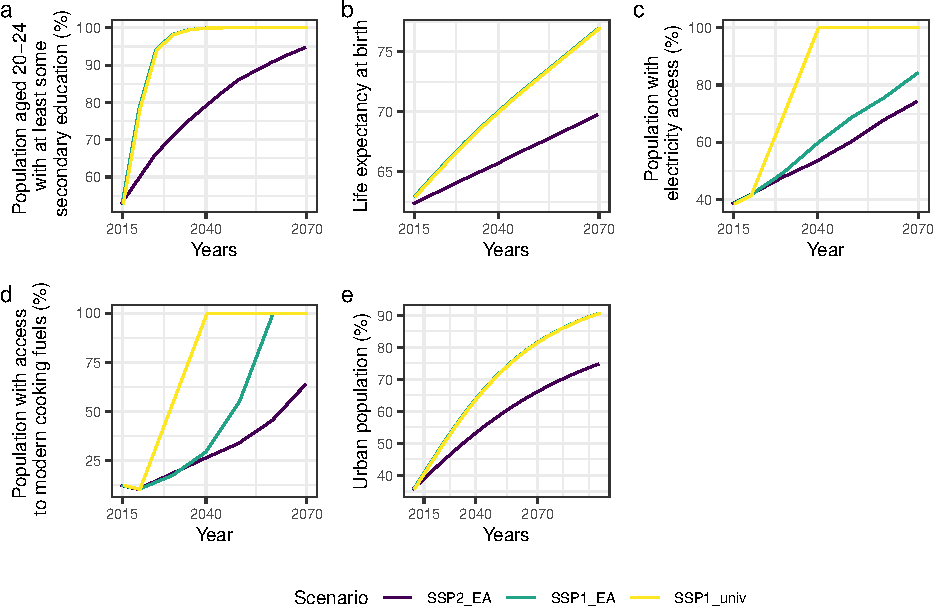
\includegraphics{../figures/input-1.pdf}
\caption{\label{fig:input}Background changes in education (a), life expectancy (b), access to electricity (c), access to modern cooking fuels (d) and urbanization (e) as input of the microsimulation model. In the case of education, life expectancy, and urbanization, the path for the SSP1\_univ scenario is the same as for \emph{SSP1\_EA}, which is why the yellow and green lines overlap in plots a, b, and e (but they were slightly dodged for visibility). On plot c and d, the distinction between rural and urban is not represented but it is taken into account in the model.}
\end{figure}

\newpage

\emph{Energy access assumptions}

The energy access assumptions we used correspond to future trajectories of the proportion of people having access to electricity and having access to modern cooking fuels. These trajectories are differentiated by rural and urban areas, to account for the important difference in energy access levels and shifts over time between rural and urban areas. The first two energy access trajectories, used in the scenarios \emph{SSP1\_EA} and \emph{SSP2\_EA}, are consistent with energy access projection by Poblete-Cazenave et al. (\protect\hyperlink{ref-poblete-cazenave_global_2021}{2021}) for the SSP1 and SSP2 pathways for the period from 2020 to 2050, that we adapted to Zambia and further projected until 2070 (Supplementary Method 4). The third and last energy access pathway we constructed is used in the scenario \emph{SSP1\_univ}, which normatively assumes universal access to both electricity and modern cooking fuels by 2040 with a linear increase in the proportion of the population having access to both forms of energy. After 2040 and until 2070, energy access remains universal. Although this scenario requires rapid percentage increases in access levels that are higher than the historical trends, in particular in rural areas where access to both forms of energy is currently very low, this normative scenario shows what would happen if the Sustainable Development Goals were achieved by 2040. From these macro-level energy access assumptions, we then derived the probability for an individual to get access to electricity, and to get access to modern cooking fuels (Supplementary Method 5).

\emph{Scenario for completely electrifying clean cooking}

In low- to middle-income countries, most households do not use only one type of cooking fuel, but often use multiple fuels, a phenomenon known as fuel stacking (\protect\hyperlink{ref-masera_linear_2000}{Masera, Saatkamp, and Kammen 2000} ; \protect\hyperlink{ref-price_stacked_2021}{Price, Barnard-Tallier, and Troncoso 2021}).
Fuel stacking can be explained by household preferences (e.g.~taste, convenience), the availability of devices and resources on local markets (\protect\hyperlink{ref-jeuland_preferences_2020}{Jeuland et al. 2020} ; \protect\hyperlink{ref-medina_understanding_2019}{Medina et al. 2019}), and as a way to secure households against shocks (e.g.~electricity outages, LPG shortages).

This phenomenon is also represented in the data we used to estimate energy consumption (see Section \ref{energyuse}). Households categorized as having access to modern cooking fuels can still have significant charcoal and firewood consumption (Figure \ref{fig:energy-use}, first and third columns), with the associated health and well-being costs.

For this reason, we created an additional scenario we referred to as \emph{SSP1\_univ\_elec}. This second normative scenario reflects a situation in which, in addition to the entire population getting access to electricity and modern cooking fuels as in \emph{SSP1\_univ}, all traditional fuel use is displaced by electricity by 2040, in line with the rapid up-scaling of electric capacity occurring concurrently in the country. To create this scenario, we used the same mortality, education, urbanization and energy access assumptions as in \emph{SSP1\_univ}, but we added a new assumption on energy consumption. To do so, we modified the energy consumption data we derived from Baltruszewicz et al. (\protect\hyperlink{ref-baltruszewicz_final_2021}{2021}) by converting traditional fuels into the equivalent electricity use, applying conversion efficiency factors of the respective fuels (Supplementary Method 6). Note that the population and fertility trajectories in the \emph{SSP1\_univ\_elec} scenario are by construction the same as in \emph{SSP1\_univ}, because in our modeling framework the energy calculator comes ex-post to the population projection model \ref{fig:overview-model}.

\newpage

\hypertarget{energyuse}{%
\subsection{Energy consumption calculator}\label{energyuse}}

The MSM estimates, for four scenarios, the population counts at each time step, broken down by education level, electricity and modern cooking fuel access as well as urbanization level. To derive the energy demand of the simulated population at each time step, we multiplied the number of people in any given category by the average per capita energy consumption of this category. We derived the latter from the study of Baltruszewicz et al. (\protect\hyperlink{ref-baltruszewicz_final_2021}{2021}). The study combines the 2015 Living Condition Measurement Survey (LCMS) for Zambia (\protect\hyperlink{ref-central_statistical_office_of_zambia_world_2015}{Central Statistical Office of Zambia 2015}) with a multi-regional input-output model to derive the energy footprint of all households surveyed. Since the household survey contains information about the education level, energy access, location of residence (urban or rural areas), we used this information to calculate the average energy consumption per capita, for households grouped along these variables (Figure \ref{fig:energy-use}). Further details on data and procedures are provided in Supplementary Method 7.

\begin{figure}
\centering
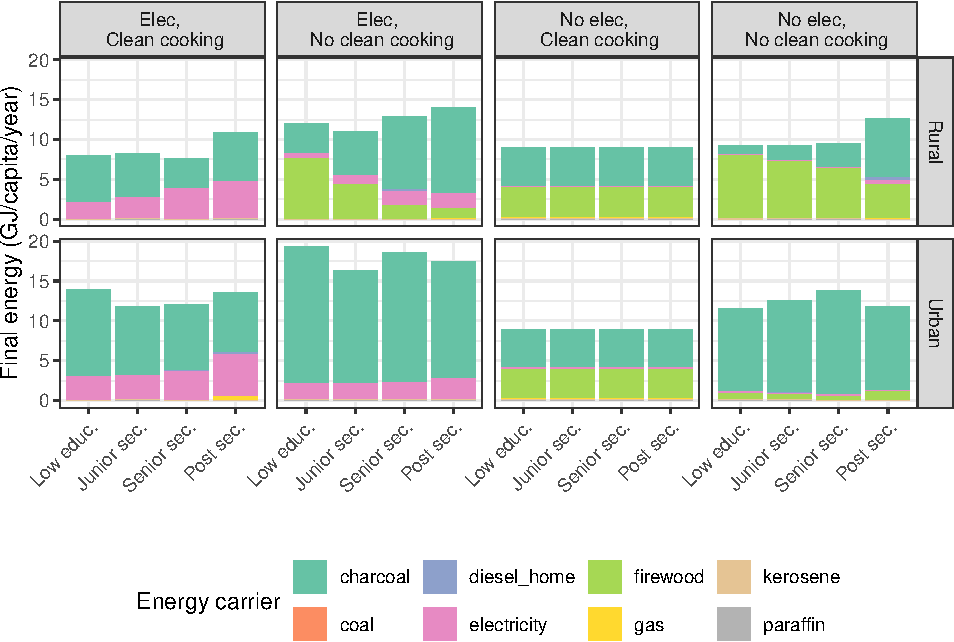
\includegraphics{../figures/energy-use-1.pdf}
\caption{\label{fig:energy-use}Energy footprints for different combination of categories in the energy-extended LCMS dataset (Baltruszewicz et al., 2021)}
\end{figure}

\newpage

\hypertarget{results}{%
\section{Results}\label{results}}

\hypertarget{population-and-fertility}{%
\subsection{Population and fertility}\label{population-and-fertility}}

We estimated that the population of Zambia in 2070 ranges from 41.5 to 54.6 to million, depending on the scenario. In scenarios where the entire population gains access to modern energy and secondary education by 2040 (\emph{SSP1\_univ}), we estimated that the population in 2070 is 27\% lower than in the baseline scenario (\emph{SSP2\_EA}) and 13\% lower than in the scenario where the entire population attains secondary education but access to modern energy remains limited (\emph{SSP1\_EA}) (Figure \ref{fig:population}, panel a). In other words, achieving universal access to modern energy reduces the population substantially compared to a more moderate expansion of energy access (\emph{SSP1\_EA}), holding all other modeling parameters (education and urbanization) constant.

The difference in population size is explained by the difference in fertility rates between the three scenarios (Figure \ref{fig:population}, panel b). In the \emph{SSP1\_univ} scenario, the total fertility rate declines almost exponentially until 2045 to reach 2.3. This corresponds to the rapid achievement of universal access to modern energy by 2040 and universal secondary education by 2030 (Figure \ref{fig:input}). The TFR continues to decline but more slowly, to drop to 1.9 in 2070. The decline in the TFR is less dramatic in \emph{SSP1\_EA} and \emph{SSP2\_EA}. In 2070, it drops to 2.4 in the \emph{SSP2\_EA} scenario and to 2.1 in \emph{SSP1\_EA}.

The population growth rate declines in all scenarios, from about 3\% in 2025 to 1.21\% in 2070 under \emph{SSP2\_EA} and to 0.69\% under \emph{SSP1\_EA} (Figure \ref{fig:population}, panel c). The population growth rate declines to 0.41\% in 2070 under \emph{SSP1\_univ}, which is similar to the value projected by WIC under SSP1 (0.34\%).

\begin{figure}
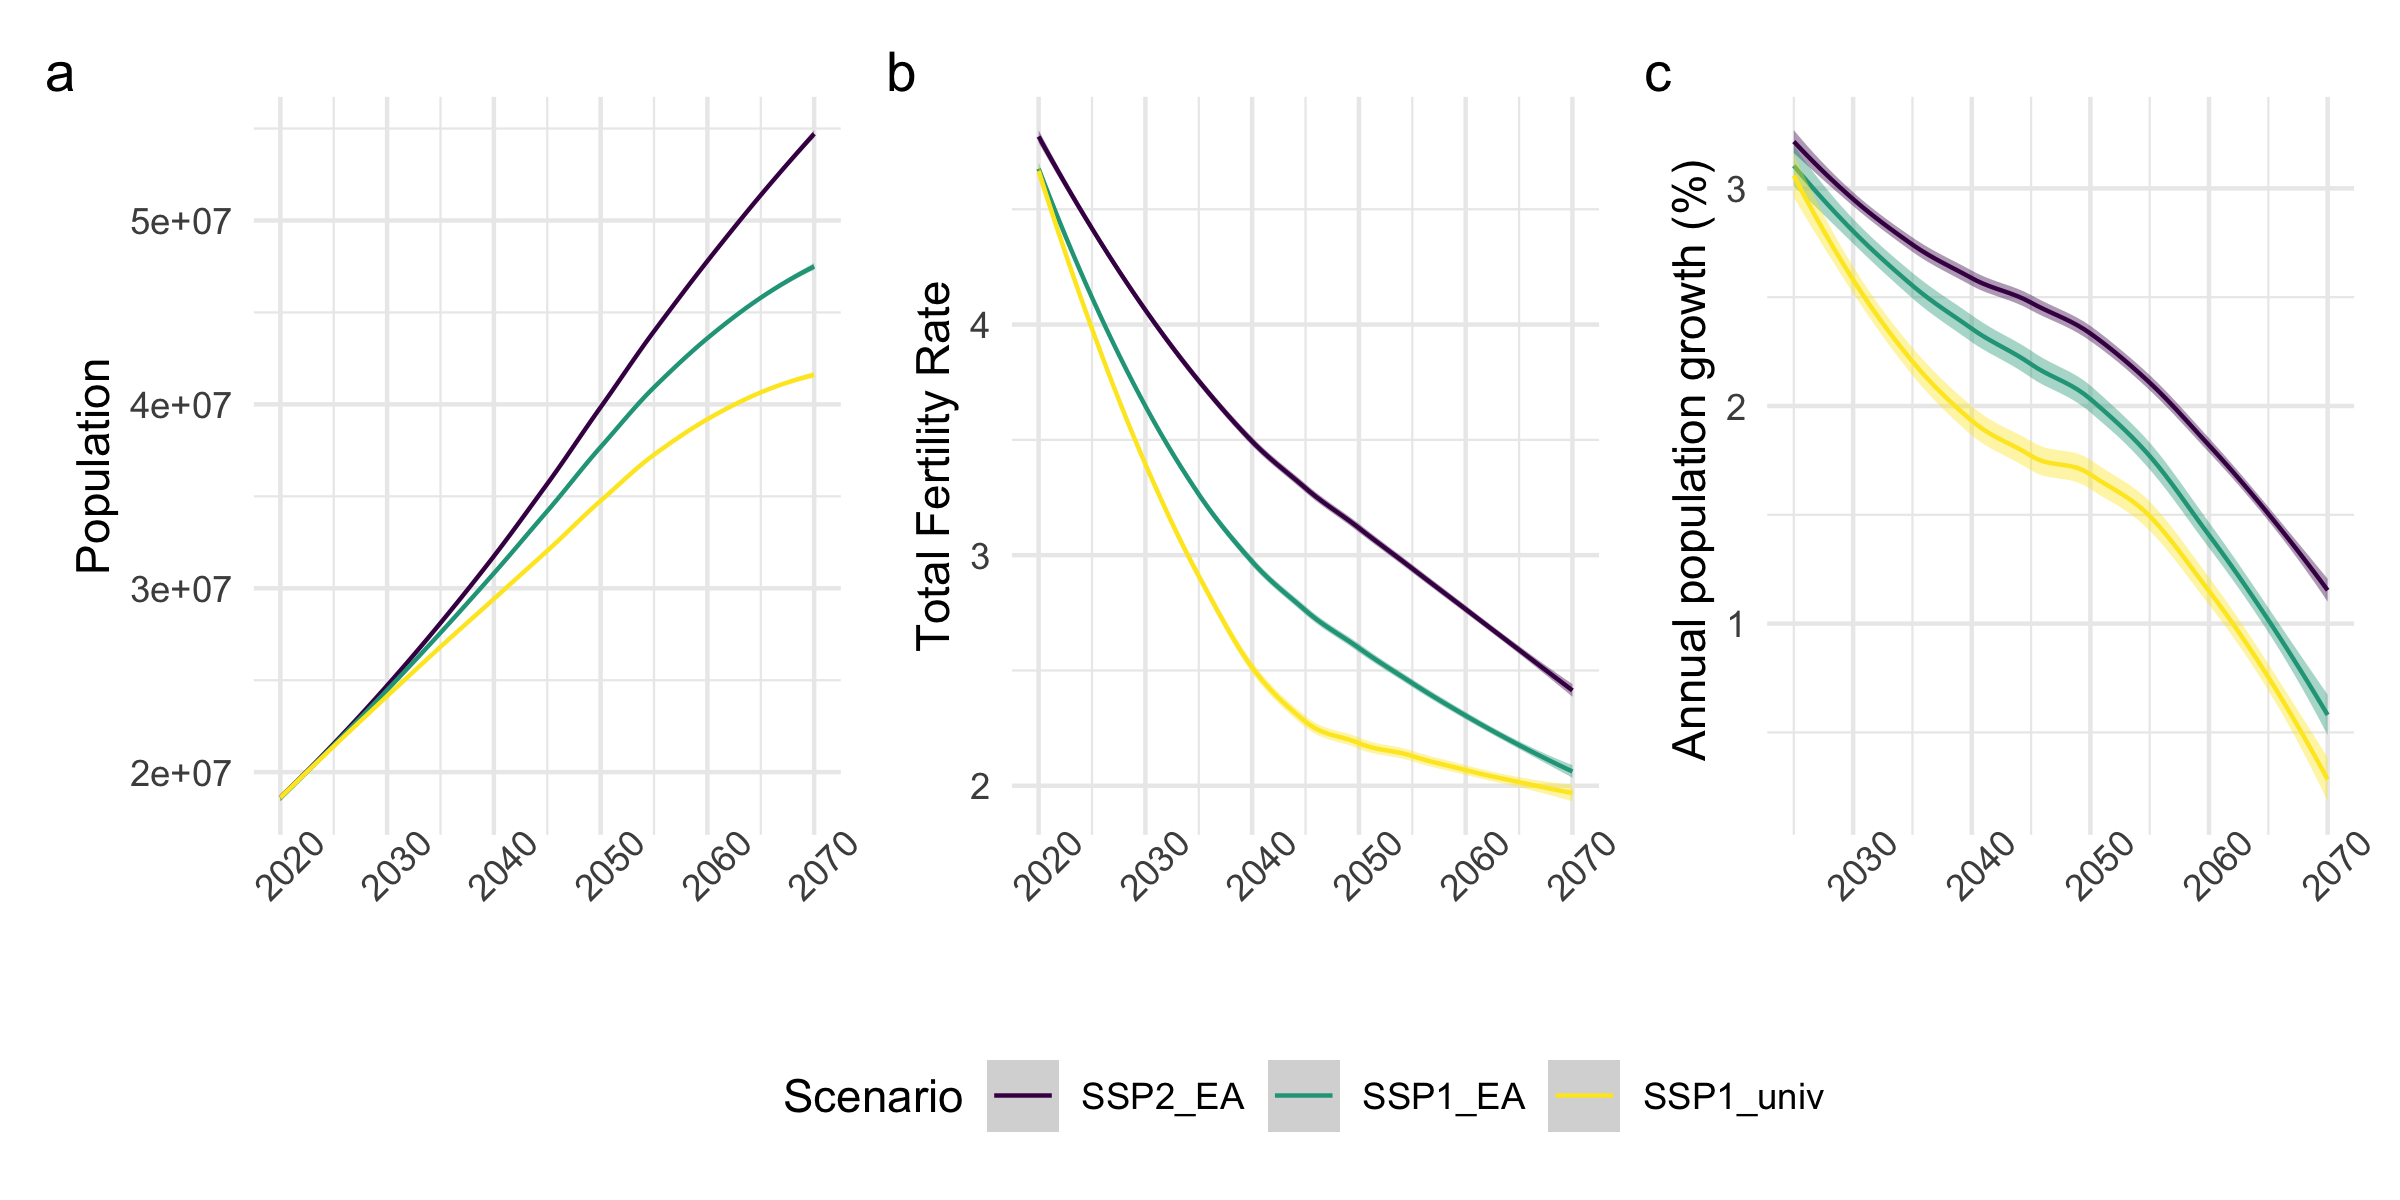
\includegraphics[width=1\linewidth]{../figures/population-1} \caption{Evolution of the population size (a), total fertility rates (c)  and annual population growth (c) in three scenarios. Note that the population and fertility trajectories for the SSP1-univ-elec are exactly the same as in SSP1-univ, by construction.}\label{fig:population}
\end{figure}

\hypertarget{energy-demand}{%
\subsection{Energy demand}\label{energy-demand}}

We estimated that the total household final energy demand of the Zambian population in 2070 ranges from to 268 to 653 PJ (Figure \ref{fig:energy-tradi-modern}). Under the \emph{SSP1\_univ} scenario, energy demand is estimated to be 29\% lower than under the \emph{SSP2\_EA} and 11\% lower than under the \emph{SSP1\_EA}. The energy demand reduction is dramatic in the \emph{SSP1\_univ\_elec} scenario, with demand being 84\% and 68\% lower than under the \emph{SSP2\_EA} and \emph{SSP1\_EA} scenarios, respectively.

In contrast to total energy demand, electricity demand is estimated to increase in all scenarios. In the baseline scenario, electricity demand in 2070 is estimated to be 8-fold higher than in 2020, reaching 109 PJ. Under both \emph{SSP1\_EA} and \emph{SSP1\_univ}, demand in 2070 is about 12-fold higher than in 2020, and it is 17 times higher in the \emph{SSP1\_univ\_elec} scenario, reaching 253PJ (Figure \ref{fig:elec}). This implies the need for a significant development of the country's installed power generation capacity.

The increase in electricity demand in our model is consistent with model results from the International Energy Agency's Africa Energy Outlook 2019. They projected electricity demand in sub-Saharan Africa (excluding South Africa) to 2040 under a \emph{Stated Policy} scenario, which simulates a situation in which all current energy policies are implemented, and an \emph{Africa Case} scenario, which reflects a situation with more ambitious goals for sustainability and economic development. They estimate that electricity demand would increase by a factor of 4 compared to 2018 levels under their \emph{Stated Policy} scenario, and by a factor of 8 under their \emph{Africa Case} scenario. These magnitudes are similar to our estimates. We estimated that by 2040, electricity demand could be as little as twice the 2020 level or as much as 10 times the 2020 level, depending on the scenario considered (Figure \ref{fig:elec} in the main text).

The share of traditional energy in the energy demand also varies strongly in the different scenarios, and in 2070 it ranges from 82\% to 59 \% (Figure \ref{fig:energy-tradi-modern}). In the \emph{SSP2\_EA} scenario, in 2070 82\% of the energy demand is traditional energy, the majority of it being firewood and charcoal. In the \emph{SSP1\_EA} scenario, 66\% comes from traditional energy, and only 59\% in the \emph{SSP1\_univ} scenario. It can be surprising that in this scenario, still more than half of the energy demand comes from traditional energy. This is explained by the fact that households use multiple fuels, and even when they get access to one source of modern energy, they continue to use some traditional energy on the side (Figure \ref{fig:energy-use}). In \emph{SSP1\_univ\_elec}, since all cooking facilities are replaced by electricity by 2040, energy demand from this date is only comprised of modern energy. The share of traditional energy in total household energy demand experiences a small drop around 2035 under \emph{SSP1\_univ} and around 2055 under \emph{SSP1\_EA}. This coincides with the timing when universal access to modern cooking fuels is achieved, which happens in 2040 under \emph{SSP1\_univ}, and in 2055 under \emph{SSP1\_EA} (Figure \ref{fig:input}).

\begin{figure}

{\centering 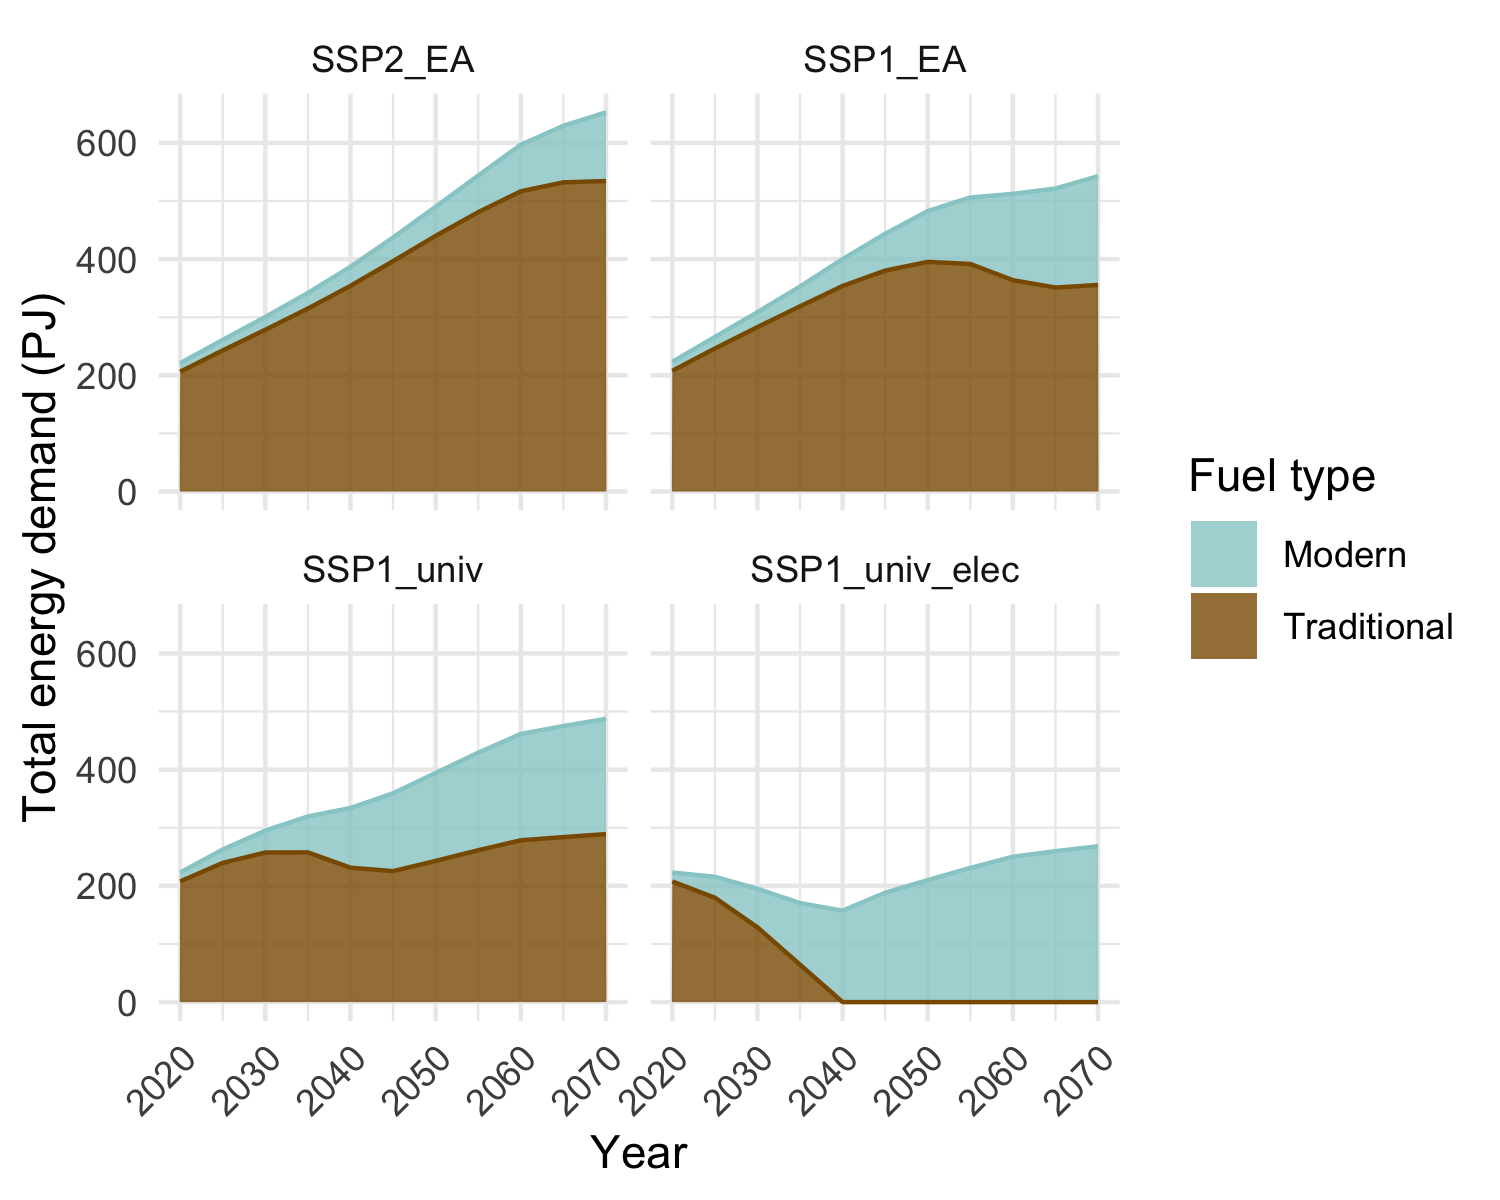
\includegraphics[width=0.8\linewidth]{../figures/energy-tradi-modern-1} 

}

\caption{Traditional and modern energy demand in the four scenarios. Traditional energy includes firewood, charcoal, coal, kerosene and paraffin. Modern energy includes electricity, gas, LPG, diesel.}\label{fig:energy-tradi-modern}
\end{figure}

\begin{figure}

{\centering 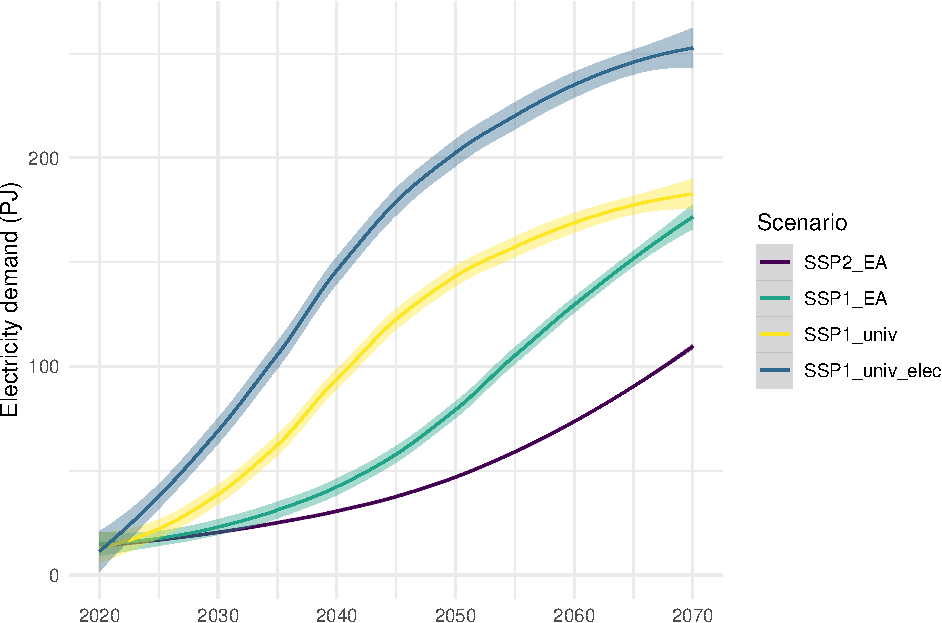
\includegraphics[width=0.6\linewidth]{../figures/elec-1} 

}

\caption{Electricity demand demand in the four scenarios.}\label{fig:elec}
\end{figure}

\hypertarget{decomposing-energy-demand-change-by-population-composition-and-size-effects}{%
\subsection{Decomposing energy demand change by population composition and size effects}\label{decomposing-energy-demand-change-by-population-composition-and-size-effects}}

The objective of this study is to quantify how projected energy demand in Zambia differs when the feedback between energy access and demographic change is taken into account compared to a case where it is not. To do so, we decomposed the growth in energy demand into the two factors that influence it: population composition and population size. First, we considered the impact on energy demand of the scenario-driven increase in the share of the population with higher education, living in urban areas, and having access to modern energy. This change in population composition affects energy consumption patterns, since energy consumption per capita differs between groups (Figure \ref{fig:energy-use}). Second, we considered the effect of changes in population size, which directly affects energy demand.

To distinguish the ``population size effect'' from the ``composition-efficiency effect'', we decomposed the change in energy demand between \emph{SSP1\_EA} and \emph{SSP1\_univ}, the two scenarios that differ only in terms of the energy access pathway. However, since the education, urbanization and mortality trajectories are identical under these two scenarios, we were able to factor out the ``population size effect'' alone.

To decompose the change in energy demand, we calculated energy demand for a hypothetical scenario in which the proportion of the population in each education, energy access, and urbanization group in each time step is kept as in \emph{SSP1\_univ}, but the population size is as in \emph{SSP1\_EA}. This simulates a situation where energy access improves, but the effect of this improvement on population size is not considered. Figure \ref{fig:energy-contrib} shows the results of this decomposition in both relative (panel a) and absolute (panel b) terms. The blue in the graph represents the composition-efficiency effect and the orange represents the population size effect.

We estimated that the ``composition efficiency'' effect due to expanded energy access contributes 25\% of the reduction in energy demand between \emph{SSP1\_EA} and \emph{SSP1\_univ} in 2030, and 55\% in 2050 (Figure \ref{fig:energy-contrib}). After 2060, this effect contributes 100\% to the total change in energy demand. In other words, if the demographic feedback is not taken into account, the energy demand under \emph{SSP1\_univ} would be higher than under \emph{SSP1\_EA} from 2060 onwards (Figure \ref{fig:energy-contrib}, panel b). Thus, the orange area represents the estimated magnitude of the overestimation of energy demand when the demographic feedback from expanded access to modern energy is not considered.

\begin{figure}
\centering
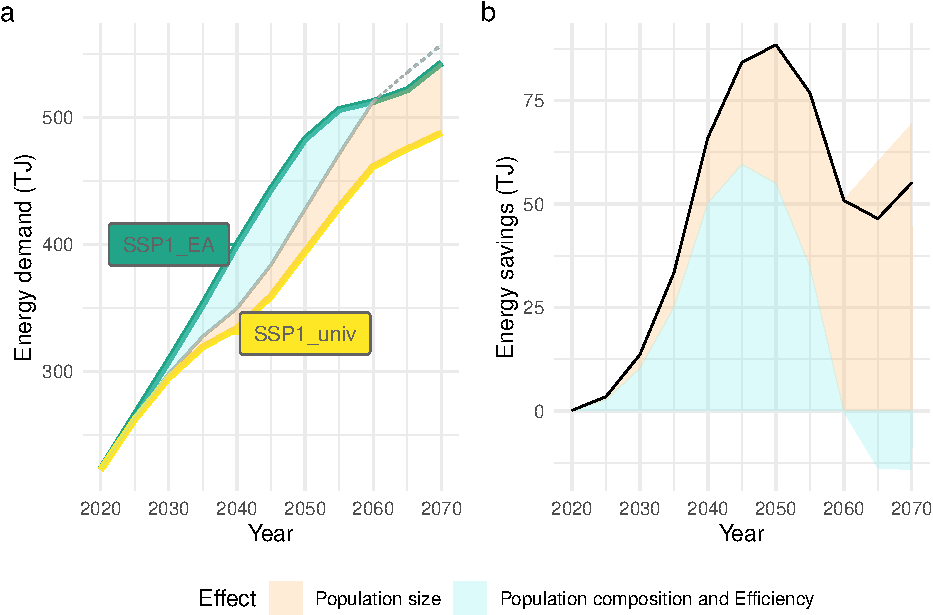
\includegraphics{../figures/energy-contrib-1.pdf}
\caption{\label{fig:energy-contrib}Decomposition of the difference in energy demand in absolute (a) and relative terms (b) between the SSP1\_univ scenario (yellow) and the SSP1\_EA scenario (green). The orange area corresponds to share of the difference in energy demand due to the population size effect (itself due to expanded energy access). The blue area represents the share of the energy demand difference that is due to the composition-efficiency effect.}
\end{figure}

\newpage

\hypertarget{discussion-and-conclusions}{%
\section{Discussion and conclusions}\label{discussion-and-conclusions}}

Achieving universal energy access is more urgent than ever. It is a necessary condition for improvements in well-being, health, education, gender equality and climate resilience, and recent studies have also shown its significant impact on reproductive health and fertility patterns. In this article, we quantified the energy demand associated with achieving universal energy access, taking into account the fact that modern energy access spurs fertility decline.

Our results suggest that improvements in living conditions and well-being can be achieved at low energy and carbon costs, and even result in energy and emissions savings. Although electricity demand is higher when the entire population of Zambia has access to modern energy compared to the baseline, household energy demand from all fuels is 29\% lower. In terms of greenhouse gas emissions, this also translates into significant differences between the scenarios. For example, emissions in the \emph{SSP1\_univ\_elec} scenario are 165\% lower than in the baseline. (Supplementary Method 8, Supplementary Tables 3-6 and Supplementary Figure 2). Implementing policies to achieve universal access to modern energy is a solution that would maximize improvements in well-being while significantly reducing emissions. If combined with climate policies that encourage the deployment of renewable energy, this would further reduce emissions (\protect\hyperlink{ref-dagnachew_trade-offs_2018}{Dagnachew et al. 2018}). This would also allow for the decarbonization of sectors other than the residential sector, which are expected to grow as the population develops.

The main contribution of this study is that it quantifies the contribution of the population effect to the observed reduction in energy demand. Typically, studies that aim to quantify the energy required to achieve universal energy access do not explicitly include the impact of energy access on population growth (\protect\hyperlink{ref-dagnachew_trade-offs_2018}{Dagnachew et al. 2018} ; \protect\hyperlink{ref-kikstra_decent_2021}{Kikstra et al. 2021} ; \protect\hyperlink{ref-rao_energy_2019}{Rao, Min, and Mastrucci 2019}). Instead, population projections such as the medium variant of the UN projection or the SSP2 scenario developed by the WIC (\protect\hyperlink{ref-kc_human_2017}{K. C. and Lutz 2017}) are used. The population size projected for Zambia in 2070 for the SSP2 scenario from the WIC is 47.1 million people, which is 13\% higher than the population size we found in the \emph{SSP1\_univ} scenario (41.5 million). Our results suggest that the estimated energy requirements for a decent life could be significantly lower if a population scenario consistent with achieving universal energy access were used. The same is true for the associated carbon and investment costs of eradicating energy poverty.

This study makes a significant contribution by providing a population projection model that endogenizes the effect of energy access on fertility. This is, to our best knowledge, unprecedented. However, there are a number of limitations that should be kept in mind when interpreting our results, and that are opportunities for future improvements. First, in the model, energy is not a predictor of mortality. This could lead to a small overestimation of the population size in scenarios with rapid improvements in energy access, as child mortality in particular declines with expansion of modern energy access (\protect\hyperlink{ref-adaji_understanding_2019}{Adaji et al. 2019}). However, as mortality depends on education, and modern energy access is correlated with education, this is unlikely to affect significantly the results.

Second, in our model, energy per capita is static for each education/modern energy access/urbanization category, whereas in reality energy consumption per wealth segment may change over time. For example, energy consumption could increase in wealthier categories due to increased demand for air conditioning as part of climate change adaptation. Energy consumption could also decrease in less affluent groups if economic and social inequalities increase. Especially since the direction of such changes is unclear, a better representation of the dynamics of energy consumption over time would be needed to better quantify the energy requirements for universal access to modern energy.

A third notable limitation is the way in which the cooking energy transition is represented. Although we know that energy-poor households tend to accumulate different fuels rather than switch from one fuel to another (fuel stacking), our model does not represent this characteristic of household energy transitions.

A third avenue for future research would be to better represent the complexity of the energy transition at the household level. This could be done by accounting for the quality of the electricity connection or better modelling the way in which the cooking energy transition occurs. For now, although we know that energy-poor households tend to accumulate different fuels rather than switch from one fuel to another (fuel stacking), our model does not represent this characteristic of household energy transitions.

More efforts are needed to incorporate the relationship between access to energy services and decent living standards and population dynamics into energy models (\protect\hyperlink{ref-kikstra_decent_2021}{Kikstra et al. 2021}). Such models can reveal novel mitigation solutions that are simultaneously beneficial to achieving other SDGs, such as SDG 7 on energy access, SDG 3 on good health, or SDG 5 on gender equality. While the challenge of rapidly achieving universal access to modern energy may seem daunting, shedding light on the additional climate co-benefits of achieving this goal could help further encourage investments aimed at achieving reliable access to modern energy for all.

\hypertarget{data-availability}{%
\section*{Data Availability}\label{data-availability}}
\addcontentsline{toc}{section}{Data Availability}

The DHS data used to produce the base population and the pooled dataset for the regression is publicly available and free of charge at: \url{https://dhsprogram.com/}, but access to the data requires a permission from the DHS Program. The WIC data is publicly available at: \url{http://dataexplorer.wittgensteincentre.org/wcde-v2/}. The raw energy data may be available upon request. The different data used to calculate greenhouse gas emissions are publicly available (see Supplementary Table 4 for all the data sources). All the available data is located on the companion git repository of this article: \url{https://github.com/camillebelmin/achieving-universal-energy-access}.

\hypertarget{code-availability}{%
\section*{Code Availability}\label{code-availability}}
\addcontentsline{toc}{section}{Code Availability}

The pre-processing and the analysis were carried out in R and Rmarkdown and are fully reproducible. All the code is available on the git repository of this article: \url{https://github.com/camillebelmin/achieving-universal-energy-access}.

\newpage

\hypertarget{references}{%
\section*{References}\label{references}}
\addcontentsline{toc}{section}{References}

\hypertarget{refs}{}
\begin{CSLReferences}{1}{0}
\leavevmode\vadjust pre{\hypertarget{ref-adaji_understanding_2019}{}}%
Adaji, Enemona Emmanuel, Winifred Ekezie, Michael Clifford, and Revati Phalkey. 2019. {``Understanding the Effect of Indoor Air Pollution on Pneumonia in Children Under 5 in Low- and Middle-Income Countries: A Systematic Review of Evidence.''} \emph{Environmental Science and Pollution Research} 26 (4): 3208--25. \url{https://doi.org/10.1007/s11356-018-3769-1}.

\leavevmode\vadjust pre{\hypertarget{ref-adhikari_ruralurban_2023}{}}%
Adhikari, Saroja, Wolfgang Lutz, and Samir Kc. 2023. {``Rural/Urban Fertility Differentials in the {Global} {South}: {Is} Female Education the Key Driver of Declining Birth Rates?''}

\leavevmode\vadjust pre{\hypertarget{ref-baltruszewicz_final_2021}{}}%
Baltruszewicz, Marta, Julia K. Steinberger, Anne Owen, Lina I. Brand-Correa, and Jouni Paavola. 2021. {``Final Energy Footprints in {Zambia}: {Investigating} Links Between Household Consumption, Collective Provision, and Well-Being.''} \emph{Energy Research \& Social Science} 73 (March): 101960. \url{https://doi.org/10.1016/j.erss.2021.101960}.

\leavevmode\vadjust pre{\hypertarget{ref-belmin_fertility_2022}{}}%
Belmin, Camille, Roman Hoffmann, Peter-Paul Pichler, and Helga Weisz. 2022. {``Fertility Transition Powered by Women's Access to Electricity and Modern Cooking Fuels.''} \emph{Nature Sustainability} 5 (3): 245--53.

\leavevmode\vadjust pre{\hypertarget{ref-central_statistical_office_of_zambia_world_2015}{}}%
Central Statistical Office of Zambia. 2015. {``World {Bank}, {Zambia} {Living} {Conditions} {Monitoring} {Survey} 2015. {Retrieved} from Http://Zambia.opendataforafrica. Org/Ssvcmrd.''}

\leavevmode\vadjust pre{\hypertarget{ref-dagnachew_trade-offs_2018}{}}%
Dagnachew, Anteneh G., Paul L. Lucas, Andries F. Hof, and Detlef P. van Vuuren. 2018. {``Trade-Offs and Synergies Between Universal Electricity Access and Climate Change Mitigation in {Sub}-{Saharan} {Africa}.''} \emph{Energy Policy} 114 (March): 355--66. \url{https://doi.org/10.1016/j.enpol.2017.12.023}.

\leavevmode\vadjust pre{\hypertarget{ref-das_virtuous_2020}{}}%
Das, Ipsita, Thomas Klug, PP Krishnapriya, Victoria Plutshack, Raja Saparapa, Stephanie Scott, Erin Sills, Marc Jeuland, Njeri Kara, and Subhrendu Pattanayak. 2020. \emph{A {Virtuous} {Cycle}? {Reviewing} the Evidence on Women's Empowerment and Energy Access, Frameworks, Metrics and Methods}.

\leavevmode\vadjust pre{\hypertarget{ref-ezzati_indoor_2005}{}}%
Ezzati, Majid. 2005. {``Indoor Air Pollution and Health in Developing Countries.''} \emph{The Lancet} 366 (9480): 104--6. \url{https://doi.org/10.1016/S0140-6736(05)66845-6}.

\leavevmode\vadjust pre{\hypertarget{ref-fuchs_education_2010}{}}%
Fuchs, Regina, Elsie Pamuk, and Wolfgang Lutz. 2010. {``Education or Wealth: Which Matters More for Reducing Child Mortality in Developing Countries?''} \emph{Vienna Yearbook of Population Research} 8: 175--99. \url{https://www.jstor.org/stable/23025514}.

\leavevmode\vadjust pre{\hypertarget{ref-fujii_fertility_2020}{}}%
Fujii, Tomoki, and Abu S. Shonchoy. 2020. {``Fertility and Rural Electrification in {Bangladesh}.''} \emph{Journal of Development Economics} 143 (March): 102430. \url{https://doi.org/10.1016/j.jdeveco.2019.102430}.

\leavevmode\vadjust pre{\hypertarget{ref-gea_global_2012}{}}%
GEA. 2012. \emph{Global {Energy} {Assessment}}. Cambridge University Press. \url{https://ideas.repec.org/b/cup/cbooks/9780521182935.html}.

\leavevmode\vadjust pre{\hypertarget{ref-grimm_does_2015}{}}%
Grimm, Michael, Robert Sparrow, and Luca Tasciotti. 2015. {``Does {Electrification} {Spur} the {Fertility} {Transition}? {Evidence} {From} {Indonesia}.''} \emph{Demography} 52 (5): 1773--96. \url{https://doi.org/10.1007/s13524-015-0420-3}.

\leavevmode\vadjust pre{\hypertarget{ref-grogan_household_2016}{}}%
Grogan, Louise. 2016. {``Household {Electrification}, {Fertility}, and {Employment}: {Evidence} from {Hydroelectric} {Dam} {Construction} in {Colombia}.''} \emph{Journal of Human Capital} 10 (1): 109--58. \url{https://doi.org/10.1086/684580}.

\leavevmode\vadjust pre{\hypertarget{ref-harbison_rural_1985}{}}%
Harbison, Sarah F., and Warren C. Robinson. 1985. {``Rural Electrification and Fertility Change.''} \emph{Population Research and Policy Review} 4 (2): 149--71. \url{https://doi.org/10.1007/BF00127549}.

\leavevmode\vadjust pre{\hypertarget{ref-icf_demographic_2004}{}}%
ICF. 2004. {``Demographic and {Health} {Surveys} {[}{Datasets}{]}. {Funded} by {USAID}.''} \url{https://dhsprogram.com/data}.

\leavevmode\vadjust pre{\hypertarget{ref-iea_weo-2016_2016}{}}%
IEA, International Energy Agency. 2016. {``{WEO}-2016 {Special} {Report}: {Energy} and {Air} {Pollution} -- {Analysis}.''} \url{https://www.iea.org/reports/energy-and-air-pollution}.

\leavevmode\vadjust pre{\hypertarget{ref-iea_tracking_2022}{}}%
IEA, IRENA, UNSD, World Bank, and WHO. 2022. {``Tracking {SDG} 7: {The} {Energy} {Progress} {Report} (2022).''} World Bank. \url{https://trackingsdg7.esmap.org/data/files/download-documents/sdg7-report2022-full_report.pdf}.

\leavevmode\vadjust pre{\hypertarget{ref-jeuland_preferences_2020}{}}%
Jeuland, Marc, Subhrendu K. Pattanayak, Jie-Sheng Tan Soo, and Faraz Usmani. 2020. {``Preferences and the {Effectiveness} of {Behavior}-{Change} {Interventions}: {Evidence} from {Adoption} of {Improved} {Cookstoves} in {India}.''} \emph{Journal of the Association of Environmental and Resource Economists} 7 (2): 305--43. \url{https://doi.org/10.1086/706937}.

\leavevmode\vadjust pre{\hypertarget{ref-jiang_global_2017}{}}%
Jiang, Leiwen, and Brian C. O'Neill. 2017. {``Global Urbanization Projections for the {Shared} {Socioeconomic} {Pathways}.''} \emph{Global Environmental Change} 42 (January): 193--99. \url{https://doi.org/10.1016/j.gloenvcha.2015.03.008}.

\leavevmode\vadjust pre{\hypertarget{ref-kc_human_2017}{}}%
K. C., Samir, and Wolfgang Lutz. 2017. {``The Human Core of the Shared Socioeconomic Pathways: {Population} Scenarios by Age, Sex and Level of Education for All Countries to 2100.''} \emph{Global Environmental Change} 42 (January): 181--92. \url{https://doi.org/10.1016/j.gloenvcha.2014.06.004}.

\leavevmode\vadjust pre{\hypertarget{ref-kikstra_decent_2021}{}}%
Kikstra, Jarmo S., Alessio Mastrucci, Jihoon Min, Keywan Riahi, and Narasimha D. Rao. 2021. {``Decent Living Gaps and Energy Needs Around the World.''} \emph{Environmental Research Letters} 16 (9): 095006. \url{https://doi.org/10.1088/1748-9326/ac1c27}.

\leavevmode\vadjust pre{\hypertarget{ref-lerch_urban_2017}{}}%
Lerch, Mathias. 2017. {``Urban and Rural Fertility Transitions in the Developing World: A Cohort Perspective.''} WP-2017-011. Rostock: Max Planck Institute for Demographic Research. \url{https://doi.org/10.4054/MPIDR-WP-2017-011}.

\leavevmode\vadjust pre{\hypertarget{ref-lutz_world_2014}{}}%
Lutz, Wolfgang, William P. Butz, and KC ed Samir. 2014. \emph{World Population and Human Capital in the Twenty-First Century}. OUP Oxford.

\leavevmode\vadjust pre{\hypertarget{ref-lutz_demographic_2018}{}}%
Lutz, Wolfgang, Anne Goujon, Samir KC, Marcin Stonawski, and Nikolaos Stilianakis. 2018. \emph{Demographic and Human Capital Scenarios for the 21st Century: 2018 Assessment for 201 Countries}. IIASA.

\leavevmode\vadjust pre{\hypertarget{ref-luzi_zambia_2019}{}}%
Luzi, Lucia, Yunhui Lin, Brian Bonsuk Koo, Dana Rysankova, and Elisa Portale. 2019. \emph{Zambia - {Beyond} {Connections}: {Energy} {Access} {Diagnostic} {Report} {Based} on the {Multi}-{Tier} {Framework}}. {ESMAP} Papers. World Bank. \url{https://doi.org/10.1596/32750}.

\leavevmode\vadjust pre{\hypertarget{ref-marois_microsimulation_2021}{}}%
Marois, Guillaume, and Samir KC. 2021. {``‪{Microsimulation} {Population} {Projections} with {SAS}: {A} {Reference} {Guide}‬.''} \url{https://scholar.google.de/citations?view_op=view_citation\&hl=fr\&user=UCjfWdcAAAAJ\&cstart=20\&pagesize=80\&citation_for_view=UCjfWdcAAAAJ:RGFaLdJalmkC}.

\leavevmode\vadjust pre{\hypertarget{ref-masera_linear_2000}{}}%
Masera, Omar R, Barbara D Saatkamp, and Daniel M Kammen. 2000. {``From {Linear} {Fuel} {Switching} to {Multiple} {Cooking} {Strategies}: {A} {Critique} and {Alternative} to the {Energy} {Ladder} {Model}.''} \emph{World Development} 28 (12): 2083--103. \url{https://doi.org/10.1016/S0305-750X(00)00076-0}.

\leavevmode\vadjust pre{\hypertarget{ref-mccollum_connecting_2018}{}}%
McCollum, David L., Luis Gomez Echeverri, Sebastian Busch, Shonali Pachauri, Simon Parkinson, Joeri Rogelj, Volker Krey, et al. 2018. {``Connecting the Sustainable Development Goals by Their Energy Inter-Linkages.''} \emph{Environmental Research Letters} 13 (3): 033006. \url{https://doi.org/10.1088/1748-9326/aaafe3}.

\leavevmode\vadjust pre{\hypertarget{ref-medina_understanding_2019}{}}%
Medina, Paulo, Victor Berrueta, Lourdes Cinco, Victor Ruiz-García, Rufus Edwards, Belén Olaya, Astrid Schilmann, and Omar Masera. 2019. {``Understanding {Household} {Energy} {Transitions}: {From} {Evaluating} {Single} {Cookstoves} to {`{Clean} {Stacking}'} {Alternatives}.''} \emph{Atmosphere} 10 (11): 693. \url{https://doi.org/10.3390/atmos10110693}.

\leavevmode\vadjust pre{\hypertarget{ref-oxfam_energy_2017}{}}%
OXFAM. 2017. {``Energy and {Women} and {Girls}: {Analyzing} the Needs, Uses, and Impacts of Energy on Women and Girls in the Developing World.''} \href{https:///explore/research-publications/energy-women-girls/}{/explore/research-publications/energy-women-girls/}.

\leavevmode\vadjust pre{\hypertarget{ref-peters_rural_2010}{}}%
Peters, Jörg, and Colin Vance. 2010. \emph{Rural {Electrification} and {Fertility}}. Essen: Rheinisch-Westfälisches Institut für Wirtschaftsforschung. \url{http://nbn-resolving.de/urn:nbn:de:101:1-20100624181}.

\leavevmode\vadjust pre{\hypertarget{ref-poblete-cazenave_global_2021}{}}%
Poblete-Cazenave, Miguel, Shonali Pachauri, Edward Byers, Alessio Mastrucci, and Bas van Ruijven. 2021. {``Global Scenarios of Household Access to Modern Energy Services Under Climate Mitigation Policy.''} \emph{Nature Energy} 6 (8): 824--33. \url{https://doi.org/10.1038/s41560-021-00871-0}.

\leavevmode\vadjust pre{\hypertarget{ref-potter_fertility_2002}{}}%
Potter, Joseph E., Carl P. Schmertmann, and Suzana M. Cavenaghi. 2002. {``Fertility and Development: Evidence from {Brazil}.''} \emph{Demography} 39 (4): 739--61. \url{https://doi.org/10.1353/dem.2002.0039}.

\leavevmode\vadjust pre{\hypertarget{ref-price_stacked_2021}{}}%
Price, Martin, Melinda Barnard-Tallier, and Karin Troncoso. 2021. {``Stacked: {In} {Their} {Favour}? {The} {Complexities} of {Fuel} {Stacking} and {Cooking} {Transitions} in {Cambodia}, {Myanmar}, and {Zambia}.''} \emph{Energies} 14 (15): 4457. \url{https://doi.org/10.3390/en14154457}.

\leavevmode\vadjust pre{\hypertarget{ref-rao_energy_2019}{}}%
Rao, Narasimha D., Jihoon Min, and Alessio Mastrucci. 2019. {``Energy Requirements for Decent Living in {India}, {Brazil} and {South} {Africa}.''} \emph{Nature Energy} 4 (12): 1025--32. \url{https://doi.org/10.1038/s41560-019-0497-9}.

\leavevmode\vadjust pre{\hypertarget{ref-riahi_shared_2017}{}}%
Riahi, Keywan, Detlef P. van Vuuren, Elmar Kriegler, Jae Edmonds, Brian C. O'Neill, Shinichiro Fujimori, Nico Bauer, et al. 2017. {``The {Shared} {Socioeconomic} {Pathways} and Their Energy, Land Use, and Greenhouse Gas Emissions Implications: {An} Overview.''} \emph{Global Environmental Change} 42 (January): 153--68. \url{https://doi.org/10.1016/j.gloenvcha.2016.05.009}.

\leavevmode\vadjust pre{\hypertarget{ref-samboko_load_2016}{}}%
Samboko, Paul, Cliff Dlamini, Kaala Moombe, and Stephen Syampungani. 2016. {``Load Shedding and Charcoal Use in {Zambia}: {What} Are the Implications on Forest Resources.''} Indaba Agricultural Policy Research Institute.

\leavevmode\vadjust pre{\hypertarget{ref-sheffield_world_1998}{}}%
Sheffield, John. 1998. {``World {Population} {Growth} and the {Role} of {Annual} {Energy} {Use} Per {Capita}.''} \emph{Technological Forecasting and Social Change} 59 (1): 55--87. \url{https://doi.org/10.1016/S0040-1625(97)00071-1}.

\leavevmode\vadjust pre{\hypertarget{ref-unfpa_world_2019}{}}%
UNFPA. 2019. {``World {Population} {Prospects} - {Population} {Division} - {United} {Nations}.''} \url{https://population.un.org/wpp/GlossaryOfDemographicTerms/}.

\leavevmode\vadjust pre{\hypertarget{ref-unfpa_world_2022}{}}%
---------. 2022. {``World {Population} {Prospects} - {Population} {Division} - {United} {Nations}.''} \url{https://population.un.org/wpp/}.

\leavevmode\vadjust pre{\hypertarget{ref-van_imhoff_microsimulation_1998}{}}%
Van Imhoff, Evert, and Wendy Post. 1998. {``Microsimulation Methods for Population Projection.''} \emph{Population} 10 (1): 97--136. \url{https://www.persee.fr/doc/pop_0032-4663_1998_hos_10_1_6824}.

\leavevmode\vadjust pre{\hypertarget{ref-who_who_2014}{}}%
WHO, -, ed. 2014. \emph{{WHO} Guidelines for Indoor Air Quality: Household Fuel Combustion}. Geneva, Switzerland: World Health Organization.

\leavevmode\vadjust pre{\hypertarget{ref-wickramasinghe_energy_2011}{}}%
Wickramasinghe, Anoja. 2011. {``Energy Access and Transition to Cleaner Cooking Fuels and Technologies in {Sri} {Lanka}: {Issues} and Policy Limitations.''} \emph{Energy Policy}, Clean {Cooking} {Fuels} and {Technologies} in {Developing} {Economies}, 39 (12): 7567--74. \url{https://doi.org/10.1016/j.enpol.2011.07.032}.

\leavevmode\vadjust pre{\hypertarget{ref-winther_womens_2017}{}}%
Winther, Tanja, Margaret N. Matinga, Kirsten Ulsrud, and Karina Standal. 2017. {``Women's Empowerment Through Electricity Access: Scoping Study and Proposal for a Framework of Analysis.''} \emph{Journal of Development Effectiveness} 9 (3): 389--417. \url{https://doi.org/10.1080/19439342.2017.1343368}.

\end{CSLReferences}

\end{document}
